% ********** Приклад оформлення пояснювальної записки **********
% *********  до атестаційної роботи ступеня бакалавра **********


\documentclass{bachelor_thesis}

% Додаткові пакети вносіть у цей файл
%%%% У даний файл додавайте всі необхідні вам додаткові пакети, наприклад...

%%%% Диаграммы
%\usepackage{tikz}                      % !!! невідомий конфлікт з якимось іншим пакетом

% Пакети для кольорових текстів (необхідні для команди \todo)
%\usepackage{xcolor}                     % !!! невідомий конфлікт з якимось іншим пакетом
%\usepackage{colortbl}

\usepackage{euscript}   %ещё один красивый шрифт \EuScript
\usepackage{listings}

%%%% ...і таке інше

%\usepackage[normalem]{ulem} % для подчёркиваний uline
%\ULdepth = 0.16em % расстояние от линии до текста выше/ниже
\usepackage[style=numeric,sorting=none]{biblatex}
\addbibresource{thesis.bib}

% Додаткові визначення та перевизначення команд вносіть у цей файл
%%% У даному файлі визначайте всі необхідні вам нові команди TeX
%%% або робіть перевизначення існуючих, наприклад...

% Перевизначення символу порожньої множини та знаків "більше-дорівнює", "менше-дорівнює" на прийняті у нас
\let\oldemptyset\emptyset
\let\emptyset\varnothing
\let\geq\geqslant
\let\leq\leqslant

% Визначення нових математичних команд
\newcommand*{\binsp}[1]{\ensuremath \left\{0, 1\right\}^{#1}}       % {0, 1}^m
\newcommand*{\xor}{\ensuremath \oplus}                              % \xor = (+)
\newcommand*{\GF}[1]{\ensuremath \mathbb F_{#1}}                    % F_n
\newcommand*{\GFgroup}[1]{\ensuremath \mathbb F^{*}_{#1}}           % F^*_n
\newcommand*{\Zring}[1]{\ensuremath \mathbb Z_{#1}}                 % Z_n
\newcommand*{\Zgroup}[1]{\ensuremath \mathbb Z^{*}_{#1}}            % Z^*_n
\newcommand*{\Jset}[1]{\ensuremath \mathbb J_{#1}}                  % J_n
\newcommand*{\Qset}[1]{\ensuremath \mathbb Q_{#1}}                  % Q_n
\newcommand*{\PQset}[1]{\ensuremath \widetilde{\mathbb Q}_{#1}}     % Q~_n
\newcommand*{\cyclic}[1]{\ensuremath \left\langle {#1} \right\rangle}                  % <g>
\newcommand*{\Legendre}[2]{\ensuremath \left( \frac{#1}{#2} \right)}  % символ Лежандра/Якоби
\newcommand*{\compinv}[1]{\ensuremath {#1}^{\left\langle -1 \right\rangle}}  % обратный по композиции

% Інший спосіб визначення математичного оператору
\DeclareMathOperator{\ord}{ord}
\DeclareMathOperator{\lcm}{lcm}
\DeclareMathOperator{\Li}{Li}
\DeclareMathOperator{\Coef}{Coef}
\DeclareMathOperator{\Log}{Log}
\DeclareMathOperator{\Exp}{Exp}
\DeclareMathOperator{\Res}{Res}
\DeclareMathOperator{\charact}{char}
\DeclareMathOperator{\Sym}{Sym}

% команда для коментарів червоним кольором
% !!! Конфлікт пакету color з якимось іншим пакетом, не використовувати
%\newcommand{\todo}[1]{\textcolor{red}{#1}}

%%% ...і таке інше

% Бюрократичні відомості про автора роботи
%%% Основні відомості %%%
\newcommand{\UDC}                      % УДК
{(впишіть правильний УДК!)}            % УДК виглядає приблизно як 004.056.5 або 513.2, або навіть 004.056.5:513.2+519.1
% Для того, щоб знайти правильний УДК, використовуйте каталог https://teacode.com/online/udc/

\newcommand{\reportAuthor}             % ПІБ автора повністю
{Нестеренко Данило Сергійович}
\newcommand{\reportAuthorShort}        % ПІБ автора коротко
{Данило НЕСТЕРЕНКО}
\newcommand{\reportAuthorGroup}        % група автора
{ФІ-01}
\newcommand{\reportTitle}              % Назва роботи
{Порівняння методiв машинного навчання для виявлення пошкоджень на сiльськогосподарських територiях}
%% використовуйте символ "\par" або "\\" для розбиття назви на декілька рядків

\newcommand{\supervisorFio}            % Науковий керівник, ПІБ повністю
{Яйлимова Ганна Олексіївна}
\newcommand{\supervisorFioShort}       % Науковий керівник, ПІБ коротко
{Ганна ЯЙЛИМОВА}
\newcommand{\supervisorRegalia}        % Науковий керівник: посада, степінь, звання
{ст. викладач каф. ММАД, д-р. філософії}              % наприклад: доцент кафедри ПЕКЛА, д.ф.-м.н., доцент
% якщо виходить дуже довго - скорочуйте: доц. каф. ПЕКЛА, д.ф.-м.н., доц.

\newcommand{\consultFio}               % Консультант, ПІБ повністю
{}
\newcommand{\consultRegalia}           % Консультант: звання, степінь, посада
{}
% Якщо у вас нема консультанта - залишайте ці поля порожніми

\newcommand{\reviewerFio}              % Рецензент, ПІБ повністю
{Яковлєв Сергій Володимирович}
\newcommand{\reviewerRegalia}          % Рецензент: звання, степінь, посада
{доц. каф. ММЗІ, к.т.н.}

\newcommand{\YearOfDefence}            % рік захисту
{2024}
\newcommand{\YearOfBeginning}          % попередній рік - може, можна це якось автоматизувати, нє?
{2023}


% Починаємо верстку документа
\begin{document}

\pagestyle{plain}
\setfontsize{14}

% Створюємо титульну сторінку
% Титульный лист
\thispagestyle{empty}
\linespread{1.1}

\begin{center}
    {\bfseries
        НАЦІОНАЛЬНИЙ ТЕХНІЧНИЙ УНІВЕРСИТЕТ УКРАЇНИ \par
        <<КИЇВСЬКИЙ ПОЛІТЕХНІЧНИЙ ІНСТИТУТ \par
        імені Ігоря СІКОРСЬКОГО>>\par
        Навчально-науковий фізико-технічний інститут\par
        \medskip
        Кафедра математичного моделювання та аналізу даних}
\end{center}

\vspace{5mm}

\begin{tabularx}{\textwidth}{XX}
     & <<До захисту допущено>>                                         \\[06pt]
     & В. о. завідувача кафедри                                        \\[06pt]
     & \rule{2.5cm}{0.25pt} Г. О. Яйлимова                             \\[06pt]
     & <<\rule{0.5cm}{0.25pt}>> \rule{2.5cm}{0.25pt} \YearOfDefence~р.
\end{tabularx}

%\linespread{1.5}                    % Неодинарный интервал
\begin{center}
    \vspace{5mm}
    {\bfseries\huge Дипломна робота} \par
    {\bfseries на здобуття ступеня бакалавра} \par
\end{center}

зі спеціальності: 113 Прикладна математика \par
на тему: \textbf{<<\reportTitle>>}

\vspace{5mm}

\begin{tabularx}{\textwidth}{>{\setlength\hsize{1.5\hsize}}X >{\setlength\hsize{0.5\hsize}}X}
    Виконав:                                  &                      \\
    студент 4 курсу, групи \reportAuthorGroup &                      \\
    \reportAuthor                             & \rule{2.5cm}{0.25pt} \\[12pt]
    Керівник:                                 &                      \\
    \supervisorRegalia                        &                      \\
    \supervisorFio                            & \rule{2.5cm}{0.25pt} \\[12pt]
    %%%%% Якщо у вас зненацька є консультант у роботі - розкоментуйте наступні три рядки (а цей - не розкоментовуйте!)
    %Консультант:                                             & \\
    %\consultRegalia                                          & \\
    %\consultFio                                              & \rule{2.5cm}{0.25pt}   \\[12pt]
    Рецензент:                                &                      \\
    \reviewerRegalia                          &                      \\
    \reviewerFio                              & \rule{2.5cm}{0.25pt}
\end{tabularx}

\vspace{15mm}

\linespread{1.1}                    % Майже одинарный интервал
\begin{tabularx}{\textwidth}{>{\setlength\hsize{1.25\hsize}}X >{\setlength\hsize{1.5\hsize}}X >{\setlength\hsize{0.25\hsize}}X}
     & Засвідчую, що у цій дипломній роботі немає запозичень з праць інших
    авторів без відповідних посилань.

     &                                                                       \\
     & Студент \rule{2.5cm}{0.25pt}                                        &
\end{tabularx}

%\vspace{10mm}
\vfill
\begin{center}
    {Київ~---~\YearOfDefence}
\end{center}

\newpage
\thispagestyle{plain}

% Створюємо завдання
% Титульный лист
\linespread{1.1}

\begin{center}
    {\bfseries
        НАЦІОНАЛЬНИЙ ТЕХНІЧНИЙ УНІВЕРСИТЕТ УКРАЇНИ \par
        <<КИЇВСЬКИЙ ПОЛІТЕХНІЧНИЙ ІНСТИТУТ \par
        імені Ігоря СІКОРСЬКОГО>>\par
        Навчально-науковий фізико-технічний інститут\par
        Кафедра математичного моделювання та аналізу даних}
\end{center}
\par

\linespread{1.1}
Рівень вищої освіти --- перший (бакалаврський)

Спеціальність --- 113~Прикладна математика,

ОПП <<Математичні методи моделювання, розпізнавання образів та комп’ютерного зору>>

\vspace{10mm}
\begin{tabularx}{\textwidth}{XX}
     & ЗАТВЕРДЖУЮ                                                      \\[06pt]
     & В.о. завідувача кафедри                                         \\[06pt]
     & \rule{2.5cm}{0.25pt} Ганна ЯЙЛИМОВА                             \\[06pt]
     & <<\rule{0.5cm}{0.25pt}>> \rule{2.5cm}{0.25pt} \YearOfDefence~р.
\end{tabularx}

\vspace{5mm}
\begin{center}
    {\bfseries ЗАВДАННЯ \par}
    {\bfseries на дипломну роботу \par}
\end{center}

%%%%%====================================
% !!! Не чіпайте наступні три команди!
%%%%%====================================
\frenchspacing
\doublespacing          % інтервал "1,5" між рядками, тепер навічно
\setfontsize{14}

Студент: \reportAuthor \par

1. Тема роботи: <<\emph{\reportTitle}>>,
науковий керівник дисертації: \supervisorRegalia ~\supervisorFio, \par
затверджені наказом по університету \No 2251-С від <<31>> травня \YearOfDefence~р.

2. Термін подання студентом роботи: <<7>> червня \YearOfDefence~р.

% Коли будете заповнювати пункти 3-10, приберіть команду \emph --- вона тільки для виділення моїх коментарів
3. Об'єкт дослідження: процес виявлення кратерів за супутниковими знімками.

4. Предмет дослідження: методи виявлення кратерів, сформованих внаслідок вибухів
бомб чи інших вибухових пристроїв, з використанням сучасних технологій обробки зображень,
супутникового зондування та геоінформаційних систем.

5. Перелік завдань: провести огляд опублікованих джерел за тематикою дослідження,
формалізувати задачу сегментації кратерів на супутникових знімках
та адаптувати до неї відомі методи розв'язання задачі сегментації,
підготувати датасет для навчання моделей машинного навчання,
провести порівняльний аналіз методів розв'язання задачі сегментації
кратерів на супутникових знімках, ґрунтуючись на створеному датасеті.

6. Орієнтовний перелік графічного (ілюстративного) матеріалу: Презентація доповіді

7. Орієнтовний перелік публікацій: виступ на XXII Всеукраїнській
науково-практичній конференції студентів, аспірантів
та молодих вчених.

8. Дата видачі завдання: 30 вересня \YearOfBeginning~р.

% Якщо перша частина завдання вилізе за сторінку - приберіть команду \newpage
% Календарний план є продовженням завдання, а не окремою частиною

\begin{center}
    Календарний план
\end{center}

\renewcommand{\arraystretch}{1.5}
\begin{table}[h!]
    \setfontsize{14pt}
    \centering
    \begin{tabularx}{\textwidth}{|>{\centering\arraybackslash\setlength\hsize{0.25\hsize}}X|>{\setlength\hsize{2\hsize}}X|>{\centering\arraybackslash\setlength\hsize{1\hsize}}X|>{\centering\arraybackslash\setlength\hsize{0.75\hsize}}X|}
        \hline \No\par з/п                                          & Назва етапів виконання магістерської дисертації & Термін виконання & Примітка \\
        \hline
        % номер етапу
        1                                                           &
        % назва етапу
        Узгодження теми роботи із науковим керівником               &
        % термін виконання
        01-15 вересня \YearOfBeginning~р.                           &
        % примітка - зазвичай "Виконано"
        Виконано                                                                                                                                    \\
        %%% -- початок інтервалу для копіювання
        \hline
        % номер етапу
        2                                                           &
        % назва етапу
        Огляд опублікованих джерел за тематикою дослідження         &
        % термін виконання
        Вересень-листопад \YearOfBeginning~р.                       &
        % примітка - зазвичай "Виконано"
        Виконано                                                                                                                                    \\
        %%% -- кінець інтервалу для копіювання
        % не прибирайте амперсанди та \\ наприкінці рядків!
        % скопійовані інтервали вставляти перед фінальною \hline та заповнювати відповідно
        % ось так:
        %%% -- початок інтервалу для копіювання
        \hline
        % номер етапу
        3                                                           &
        % назва етапу
        Огляд моделей машинного навчання та функцій втрат           &
        % термін виконання
        Листопад \YearOfBeginning~р.-січень \YearOfDefence~р.       &
        % примітка - зазвичай "Виконано"
        Виконано                                                                                                                                    \\
        %%% -- кінець інтервалу для копіювання
        \hline
        % номер етапу
        4                                                           &
        % назва етапу
        Імплементація та тренування моделей машинного навчання      &
        % термін виконання
        Січень-квітень \YearOfDefence~р.                            &
        % примітка - зазвичай "Виконано"
        Виконано                                                                                                                                    \\
        \hline
        % номер етапу
        5                                                           &
        % назва етапу
        Проведення порівняльного аналізу моделей машинного навчання &
        % термін виконання
        Квітень-травень \YearOfDefence~р.                           &
        % примітка - зазвичай "Виконано"
        Виконано                                                                                                                                    \\
        \hline
        % номер етапу
        6                                                           &
        % назва етапу
        Оформлення дипломної роботи                                 &
        % термін виконання
        Травень-14 червня \YearOfDefence~р.                         &
        % примітка - зазвичай "Виконано"
        Виконано                                                                                                                                    \\
        \hline %фінальна hline
    \end{tabularx}
\end{table}

\renewcommand{\arraystretch}{1}
\begin{tabularx}{\textwidth}{>{\setlength\hsize{1.2\hsize}}X >{\setlength\hsize{0.5\hsize}}X >{\setlength\hsize{1.3\hsize}}X}
    Студент  & \rule{2.5cm}{0.25pt} & \reportAuthorShort  \\[06pt]
    Керівник & \rule{2.5cm}{0.25pt} & \supervisorFioShort \\
\end{tabularx}

\newpage


% У даному костильному рішенні перші три сторінки (титул та завдання на 
% роботу) друкуються окремо від основної частини тез.
% Тому перша сторінка сформованого документу нумерується як четверта

% Створюємо анотації
%\setcounter{page}{4}
%!TEX root = ../abstract.tex

\abstractUkr

Кваліфікаційна робота містить: 50 стор., 7 рисунків, 1 таблицю, 19 джерел.

Метою дослідження є уточнення методів
розв'язання задачі сегментації кратерів на супутникових знімках
на основі моделей машинного навчання.
Об'єктом дослідження є процес виявлення кратерів за супутниковими знімками.
Предметом дослідження є методи виявлення кратерів, сформованих
внаслідок вибухів бомб чи інших вибухових пристроїв, з використанням
сучасних технологій обробки зображень, супутникового зондування та
геоінформаційних систем.

Під час дослідження було проведено аналіз та порівняння
існуючих методів розв'язання задачі сегментації на супутникових
зображеннях. Використання результатів поставлених задач роботи
можуть бути застосовані для оцінки пошкоджень, визначення
найбільш вразливих зон для населення, тощо. Результати
дослідження показали, що модель U-Net з використанням Dice
Loss виявилася найбільш ефективною, здатною точно визначити
місцеположення кратерів. Також, виявлено, що моделі, навчені з
використанням Dice Loss, показали кращі та стабільніші результати
порівняно з моделями, навченими з використанням Focal Loss.

% наприкінці анотації потрібно зазначити ключові слова
Ключові слова: \MakeUppercase{машинне навчання, u-net, fpn, deeplabv3}

%%%% Рішенням кафедри з 2018 року ми прибираємо анотації російською мовою
% \abstractRus
%
%Русская аннотация должна быть точным переводом украинской (включая 
%статистику и ключевые слова).

\abstractEng

Qualification work contains: 50 pages, 7 figures, 1 table, 19 sources.

The purpose of the study is to refine methods for solving the problem of crater
segmentation on satellite images based on machine learning models. The object
of research is the process of detecting craters from satellite images. The
subject of the study is the methods of detecting craters formed as a result of
bombings or other explosive devices using modern image processing technologies,
satellite sensing and geographic information systems.

The study analyzed and compared existing methods for solving the segmentation
problem on satellite images. Using the results of the set tasks, the work can
be applied to damage assessment, identification of the most vulnerable areas
for the population, etc. The results of the study showed that the U-Net model
using Dice Loss proved to be the most effective, able to accurately determine
the location of craters. It was also found that the models trained using Dice
Loss showed better and more stable results compared to the models trained using
Focal Loss.

Keywords: \MakeUppercase{machine learning, u-net, fpn, deeplabv3}

% Не прибирайте даний рядок
\clearpage

% Створюємо зміст
%\pagenumbering{gobble}
\tableofcontents
\cleardoublepage
%\pagenumbering{arabic}
%\setcounter{page}{1}    %!!! -- продумати, як автоматизувати номер сторінки

% Створюємо перелік умовних позначень, скорочень і термінів
% Якщо цей розділ вам не потрібен, просто закоментуйте два наступних рядка
\shortings
%!TEX root = ../thesis.tex
% створюємо перелік умовних позначень, скорочень і термінів
\begin{tabbing}
    \hspace{0.8in}\=\hspace{1in}\=\kill

    \textit{MPP} \>--- Marked Point Process \\

    \textit{CNN} \>--- Convolutional Neural Network (згорткова нейронна мережа) \\

    \textit{FPN} \>--- Feature Pyramid Networks \\

    \textit{IoU} \>--- Intersection over Union \\

    \textit{Recall} \>--- повнота \\

    \textit{Precision} \>--- точність \\
\end{tabbing}

% Створюємо вступ
\intro
%!TEX root = ../thesis.tex
% створюємо вступ
% \textbf{Актуальність дослідження.}
Повномасштабне вторгнення
в Україну призвело до значних ушкоджень сільськогосподарських угідь.
Деформація ґрунтового покриву внаслідок формування фортифікаційних
споруд (окопів), утворення кратерів від бомб, хімічне забруднення внаслідок
використання боєприпасів –- це лише короткий перелік наслідків вторгнення~\cite{golubtsov2023}.
Задача даної робити -- проаналізувати існуючі методи розв'язання задачі сегментації
на супутникових зображеннях і виявити найбільше ефективного.
Використання результатів поставлених задач роботи можуть бути застосовані для оцінки пошкоджень,
визначення найбільш вразливих зон для населення, тощо.

\textbf{Метою дослідження} є уточнення методів
розв'язання задачі сегментації кратерів на супутникових знімках
на основі моделей машинного навчання.
Для досягнення мети необхідно розв'язати наступні \textbf{задачі дослідження}:

\begin{enumerate}
    \item провести огляд опублікованих джерел за тематикою дослідження;
    \item формалізувати задачу сегментації кратерів на супутникових знімках
          та адаптувати до неї відомі методи розв'язання задачі сегментації;
    \item підготувати датасет для навчання моделей машинного навчання;
    \item провести порівняльний аналіз методів розв'язання задачі сегментації
          кратерів на супутникових знімках, ґрунтуючись на створеному датасеті.
\end{enumerate}

\emph{Об'єктом дослідження} є процес виявлення кратерів за супутниковими знімками.

\emph{Предметом дослідження} є методи виявлення кратерів, сформованих внаслідок вибухів
бомб чи інших вибухових пристроїв, з використанням сучасних технологій обробки зображень
та моделей машинного навчання.

% Додаємо глави
% Якщо ваша робота містить менше або більше глав - модифікуйте наступні 
% рядки відповідним чином
%!TEX root = ../thesis.tex

\chapter{Постановка задачі дослідження та огляд існуючих методів її розв'язання}
\label{chap:review}  %% відмічайте кожен розділ певною міткою -- на неї наприкінці необхідно посилатись

\section{Метод Marked Point Processes}

Одним з сучасних методів визначення кратерів на супутникових
знімках є робота~\cite{mpp2022}. У статті представлено
стохастичний підхід, заснований на процесах маркованих
точок (MPP) для автоматичного виявлення бомбових
воронок на аерофотознімках воєнного часу. Метод
використовує виявлені воронки для створення карти
впливу, яка класифікує території як потенційно забруднені
або незабруднені на основі ймовірності наявності
нерозірваних боєприпасів. Підхід було протестовано
на знімках з Нижньої Саксонії, Зальцбурга та Італії,
причому оцінювання проводилося як на основі об'єктів,
так і на основі пікселів. Експерименти були зосереджені
на аналізі моделі, впливу різних параметрів і порівнянні
з об'єктним детектором на основі глибокого навчання.

При аналізі моделі порівнювалися результати, отримані
при використанні кола та еліпса в якості об'єктної моделі.
Було виявлено, що при використанні еліпса дещо підвищується
повнота, але знижується точність, що робить
модель кола більш стабільною.

F1 score -- це показник, який використовується в статистичному аналізі для
оцінки точності тесту на бінарну класифікацію. Це середнє гармонійне значення
точності та повноти, що забезпечує баланс між цими двома показниками. Це робить
його особливо корисним в ситуаціях, коли потрібно знайти баланс між точністю
(точністю позитивних прогнозів) і повнотою (здатністю знайти всі позитивні
приклади).

Дослідження також оцінило важливість різних енергетичних доданків у моделі,
показавши, що виключення певних доданків призводило
до збільшення кількості хибних спрацьовувань і зменшення
показника F1. Результати продемонстрували ефективність
запропонованої моделі для точного виявлення бомбових кратерів.

У дослідженні також вивчався вплив використання надлишкової
інформації зображення шляхом об'єднання результатів виявлення
з декількох зображень, що покривають одну і ту ж ділянку.
Результати показали значне покращення показника F1 при
об'єднанні результатів виявлення, що вказує на потенціал
використання декількох зображень для підвищення точності
виявлення. Крім того, дослідження було зосереджено на
оптимізації точності результатів, що має вирішальне
значення для запропонованого сценарію застосування,
шляхом варіювання параметрів для досягнення більш високої
точності за рахунок повноти.

Порівняння підходу MPP з детектором об'єктів на основі
глибокого навчання показало, що модель глибокого
навчання перевершує підхід MPP в сценаріях з достатньою
кількістю маркованих навчальних даних. Однак у сценаріях
з обмеженою кількістю мічених даних або взагалі без них
підхід MPP показав кращі результати. Дослідження підкреслило
перевагу підходу на основі моделей у сценаріях, де навчальних
даних недостатньо або вони взагалі відсутні, що дозволяє
уникнути необхідності великого ручного маркування.

Загалом, результати дослідження продемонстрували ефективність
підходу MPP в автоматичному виявленні вирв від бомб на
аерофотознімках воєнного часу. Метод показав багатообіцяючі
результати у позначенні зон впливу з високою точністю.
У той же час, метод не найкращим чином придатний для точного
виявлення кратерів на знімках.

\section{Підхід з використанням CNN}

Згорткові нейронні мережі (CNN)~\cite{oshea2015} -- це тип штучних
нейронних мереж,
який зазвичай використовується для аналізу візуальних даних,
таких як зображення. Вони отримали свою назву
через використання операції згортки, яка є основною
для виявлення візуальних шаблонів або функцій у вхідних даних.
Одна з ключових особливостей CNN -- це використання шарів згортки
та пулінгу, які допомагають зменшити кількість параметрів у мережі
і забезпечують роботу з об'єктами різних розмірів у вхідних даних.

Згорткові нейронні мережі широко застосовуються в різних задачах
обробки зображень, таких як розпізнавання об'єктів, класифікація
зображень, виявлення облич, а також у задачах комп'ютерного зору.
Їхній успіх полягає в здатності автоматично вивчати корисні функції
зображень з великою кількістю даних для тренування, що робить їх
ефективним інструментом у багатьох сферах, включаючи медицину,
автомобільну промисловість та аналітику зображень.

Робота~\cite{clermont2019} використовує CNN для розв'язання задачі
бінарної класифікації, тобто по зображенню визначає, чи є на ньому кратер,
чи це фонове зображення.

На рисунку~\ref{cnn_paper_arch} зображена кінцева архітектура мережі. Як видно,
до готового екстрактора підключені два повнозв'язних шари, які потім підключені
до ще одного softmax шару. Під час тренування, оновлюються ваги останніх двох
шарів попередньо навченої мережі (Block 8 і шар FC), а також шари, додані
авторами.

\begin{figure}[ht]
      \centering
      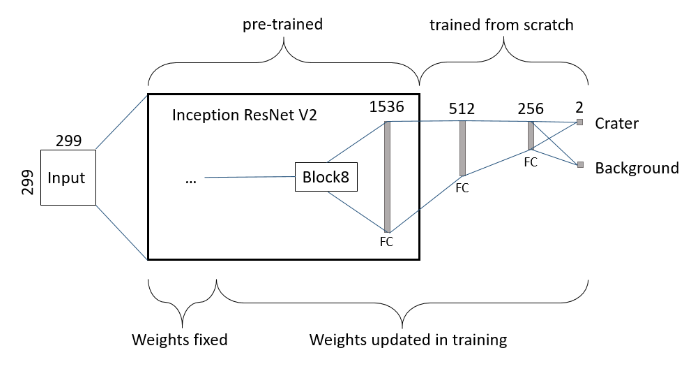
\includegraphics[scale=0.75]{Images/paper_arch.png}
      \caption{Архітектура мережі, запронованої у роботі~\cite{clermont2019}}
      \label{cnn_paper_arch}
\end{figure}

У статті представлено метод контрольованого виявлення вирв
від бомб на історичних аерофотознімках з використанням
згорткових нейронних мереж (CNN). Метою дослідження є
автоматичне виявлення кратерів від бомб на знімках часів
Другої світової війни для відстеження бомб, що не розірвалися,
які все ще становлять загрозу сьогодні. Метод складається з
двох основних етапів: вилучення кандидатів у кратери за
допомогою детектора блобів (від англ. blob, що в даному контексті
означає форму кратера) і класифікація цих кандидатів
як кратерів або фону за допомогою CNN. Підхід має
на меті покращити виявлення кратерів від бомб на
історичних знімках, що може бути складним завданням
через варіації зовнішнього вигляду кратерів та неточності
в довідкових анотаціях.

Експерименти, проведені в дослідженні, виявили цікаві
результати. Процес виділення кандидатів за допомогою
детектора блобів показав, що метод не може досягти необхідної
точності, вказуючи на те, що не всі еталонні кратери
були виділені як кандидати. Це може бути пов'язано з
обмеженнями обраних параметрів блоб-детектора, оскільки
деякі кратери на зображеннях не мали чіткого блобоподібного
вигляду. Крім того, порівняння з методом ковзного вікна
показало необхідність подальшої оптимізації параметрів
для покращення процесу виділення кандидатів.

З точки зору класифікації, експерименти продемонстрували
вплив ваги помилкових спрацьовувань на результати.
Використання ваги, що відповідає співвідношенню позитивних
і негативних вибірок, значно покращило показник F1,
що вказує на важливість балансування помилок класифікації.
Однак переносимість між наборами даних була не такою успішною:
CNN показала кращі результати на тому наборі даних,
на якому вона навчалась. Це свідчить про те,
що відмінності між наборами даних і неточності
в довідкових анотаціях можуть впливати на результати класифікації.

У дослідженні також вивчалося поєднання наборів
даних для покращення результатів класифікації. Хоча навчання
і тестування на комбінованому наборі даних не дало кращих
результатів порівняно з навчанням на окремих наборах даних,
необхідні подальші дослідження, щоб зрозуміти вплив відмінностей
у наборах даних на роботу CNN. Результати свідчать про те,
що CNN може мати труднощі з перенесенням знань між наборами
даних з різними характеристиками, що підкреслює необхідність
застосування методів адаптації до предметної області для
підвищення точності класифікації. Загалом, дослідження дає
цінну інформацію про виклики і можливості автоматизованого
виявлення вирв від бомб на історичних аерофотознімках за
допомогою CNN. В той же час, результати виявилась недостатньо
гарними для того, щоб назвати запропоновану архітектуру
точною та ефективною. Крім того, дана модель використовується
лише для класифікації зображень, а не для сегментації.

\section{Методи, засновані на статистичних індикаторах}

Роботи~\cite{mikava2023,shelestov2023} виявляють та аналізють пошкодження
територій за допомогою
індексу рослинності NDVI, при цьому інформація оцінюється
за певні часові інтервали.

Дослідження фокусується на виявленні типових пошкоджень,
таких як воронки від обстрілів і вибухів, вигорілі поля
та сліди військової техніки. Оцінці втрат від конфлікту в
Україні присвячено багато робіт, в яких застосовуються
різні методи -- від виявлення воронок до оцінки пошкоджень
міських територій. Супутникові дані, зокрема місії
Sentinel-2, відіграють вирішальну роль у цьому аналізі.

Методологія передбачає розрахунок
індексу NDVI та аналіз спектральних каналів для виявлення
пошкоджених сільськогосподарських угідь. У дослідженні
оцінка поділяється на двотижневі періоди і порівнюються
значення NDVI до і після конкретних подій для точного
моніторингу пошкоджень. Результати показують, що метод,
заснований на відносній різниці у значеннях NDVI, дозволяє
виявити значно більшу кількість пошкоджених полів порівняно
з візуальною оцінкою.

Валідація методу включала візуальну перевірку вибраних
ділянок і порівняння з оперативними даними ACLED.
Дослідження успішно виявило пошкоджені поля в Донецькій області,
що відповідає офіційним повідомленням про обстріляні території.
Метод виявився ефективним у виявленні пошкоджень, особливо
в районах, близьких до зон активних бойових дій.

До переваг запропонованого методу виявлення пошкоджень
сільськогосподарських угідь з використанням супутникових
даних та вегетаційного індексу NDVI можна віднести наступні:

\begin{itemize}

      \item Об'єктивна оцінка: Метод забезпечує
            об'єктивну оцінку пошкоджень на основі
            кількісних даних, що зменшує ймовірність
            упередженості в оцінках.
      \item Масштабованість: Метод можна
            застосовувати в різних масштабах,
            від окремих полів до великих регіонів,
            що робить його універсальним для різних рівнів аналізу.

\end{itemize}

До недоліків запропонованого методу можна віднести:

\begin{itemize}

      \item Сезонна мінливість: Сезонні
            зміни рослинності та умов навколишнього
            середовища можуть впливати на значення NDVI,
            що вимагає ретельного розгляду і потенційно
            впливає на точність виявлення пошкоджень.
      \item Верифікація: Хоча метод забезпечує
            автоматизоване виявлення пошкоджень,
            для підтвердження точності результатів може
            знадобитися ручна перевірка, що додає додатковий
            етап до процесу.
      \item Доступність даних: Ефективність
            методу залежить від наявності високоякісних
            супутникових даних, які не завжди можуть
            бути постійно доступними або актуальними в
            регіонах, що постраждали від конфлікту.

\end{itemize}

Загалом, хоча запропонований метод пропонує значні переваги
в оцінці збитків, завданих сільськогосподарським угіддям,
важливо враховувати ці обмеження, щоб забезпечити точність
і достовірність результатів.

Ще одним прикладом застосування індексу NDVI є робота~\cite{deininger2023}, у якій
NDVI використовується для оцінки врожайності полів озимих зернових. Результати
показують, що даний метод є ефективним для оцінки пошкоджень такого типу.

Робота~\cite{kussul2023} представляє комплексну методологію автоматичної ідентифікації
сільськогосподарських територій, пошкоджених діями у воєнний
час, з використанням супутникових даних Sentinel-2.

Методологія, описана в статті, передбачає використання
спектральних смуг з роздільною здатністю 10 м та
індексів рослинності з даних Sentinel-2,
а також статистичних показників за певний проміжок часу,
як вхідних даних для класифікатора Random forest.
Алгоритм ефективно визначає пошкоджені поля з високою
точністю близько 0.85. Потім використовується підхід
виявлення аномалій для окреслення пошкоджень в межах
полів шляхом поєднання спектральних смуг та індексів.

У статті~\cite{kussul2023} використані наступні статистичні показники:

\begin{itemize}

      \item NDVI -- це загальновизнаний вегетаційний індекс, який вимірює стан і щільність
            рослинності. У дослідженні NDVI використовується для виявлення аномалій у
            рослинному покриві, особливо у відповідь на пошкодження, спричинені військовою
            діяльністю.
      \item EVI -- це ще один вегетаційний індекс, який використовується для оцінки
            здоров'я та щільності рослинності. У цьому дослідженні EVI розглядається разом
            з NDVI для оцінки впливу пошкоджень на сільськогосподарські поля.
      \item AVI -- це вегетаційний індекс, який включає в себе певні спектральні діапазони
            для оцінки здоров'я та життєздатності рослинності. Він використовується в
            дослідженні для доповнення аналізу пошкоджень на сільськогосподарських полях.
      \item GCI -- це вегетаційний індекс, який фокусується на вмісті хлорофілу в
            рослинності. У дослідженні GCI використовується для виявлення аномалій у
            рослинному покриві та оцінки пошкоджень сільськогосподарських полів.

\end{itemize}

Дослідження, проведене протягом 22
двотижневих періодів у 2022 році, виявило
близько 500 тисяч гектарів орних земель у
10 регіонах України, які були пошкоджені. Результати методології
демонструють ефективність автоматизованого супутникового
моніторингу для оцінки впливу військових дій на сільське
господарство.

Ще одним індексом, який можна використати для визначення пошкоджень,
є NDWI -- індекс дистанційного зондування, який використовується
для визначення та моніторингу наявності водних об'єктів,
вмісту води в рослинності та змін у вмісті води в рослинному покриві~\cite{kussul20232}.
Підхід було застосовано на тестовій ділянці площею 8 800
га в Донецькій області. Використовуючи знімки PlanetScope
з роздільною здатністю 3 метри, автори змогли виявити 202 гектари
кратерів, що становить 63\% від виявлених на знімках SkySat.
На знімках Sentinel-2 з роздільною здатністю 10 метрів автори
виявили 165 гектарів кратерів, або 51\% від тих, що були
виявлені на знімках SkySat.

\section{Постановка задачі}

Основною задачею є розробка автоматизованого методу точної
сегментації та ідентифікації кратерів від вибухів бомб на супутникових
знімках. Цей метод спрямований на покращення виявлення,
моніторингу та аналізу наслідків вибухів бомб у зонах
конфліктів для гуманітарних та екологічних цілей.
Кратер -- це кругла або майже кругла заглибина,
що утворилася на поверхні землі внаслідок падіння та
вибуху бомби. Кратери зазвичай мають такі характеристики:
переважно круглу або еліптичну форму, підняті краї по
периметру, часто зі зміщеним ґрунтом або уламками,
помітну глибину порівняно з навколишньою місцевістю
а також виразні відмінності в текстурі всередині кратера
і в безпосередній близькості від нього, зумовлені вибуховою хвилею від вибуху.

Вхідні дані для цієї задачі складаються зі знімку та маски. Методологія включає в себе
декілька кроків. Спочатку треба підготувати датасет, фрагментуючі вхідні дані, для
отримання достатньої кількості навчального та тестового матеріалу. Наступним кроком
є імплементація моделей машинного навчання, навчання їх на тестовому датасеті
та отримання відповідних метрик, за якими потім буде проводитися
порівняльний аналіз моделей.

Метрики моделі включають точність, повноту, IoU та F1. За даними метриками
можна точно визначити моделі, які краще справляються з розв'язанням
задачі сегментації кратерів на супутникових знімках.

\section*{Висновки до розділу 1}

Отже, у даному розділі було проведено огляд існуючих методів
розв'язання задачі дослідження та формалізовано задачу
сегментації кратерів на супутникових знімках.
У приведених роботах використовувалися різні підходи, а саме MPP, CNN, та
методи, засновані на використанні статистичних показників.
MPP показав свою ефективність у розв'язуванні цієї задачі, особливо
за умов, коли немає розміченої маски, або коли даних недостатньо для
тренування більш складної CNN моделі. Методи, засновані
на статистичних показниках теж потребують менше даних за CNN,
але потрібні знімки, розподілені у часі, що може ускладнити успішне використання
цього методу.
У той же час, якщо даних достатньо,
то CNN дає більш точні результати.

У ході формалізації завдання було дано визначення поняттю кратера,
описані вхідні дані, кроки методології та метрики, за якими будуть
порівнюватися моделі машинного навчання.
%!TEX root = ../thesis.tex
% створюємо розділ
\chapter{Огляд моделей машинного навчання навчання та функцій втрат}
\label{chap:theory}

\section{Модель Feature Pyramid Networks}

FPN (Feature Pyramid Networks) -- це інструмент для виділення ознак, який
приймає на вхід одномасштабне зображення довільного розміру, а на вихід подає
карти ознак пропорційного розміру на декількох рівнях, повністю згорнуті за
допомогою методу згортки~\cite{lin2016}. Цей процес не залежить від базової
згорткової архітектури. Тому він діє як загальне рішення для побудови пірамід
ознак всередині глибоких згорткових мереж для використання в таких задачах, як
виявлення об'єктів.

FPN -- це передова архітектура, яка широко використовується в задачах
комп'ютерного зору, зокрема, для виявлення та сегментації об'єктів. Архітектура
FPN вирішує проблему виявлення об'єктів різного масштабу шляхом створення
різномасштабного представлення ознак з одного вхідного зображення. Це
досягається за допомогою ієрархічного підходу, який використовує властиву
згортковим нейронним мережам (CNN) форму піраміди. Основна ідея полягає в тому,
щоб будувати карти об'єктів з різною роздільною здатністю, фіксуючи дрібні
деталі з високою роздільною здатністю і більш абстрактні об'єкти з низькою
роздільною здатністю, що дозволяє надійно виявляти об'єкти різного розміру.

Загальна архітектура мереж FPN зображена на рис.~\ref{fpn_arch}. FPN складається з двох основних частин: висхідного шляху та низхідного шляху з
бічними зв'язками. Висхідний шлях -- це стандартна згорткова мережа, яка
створює карти ознак з меншою просторовою роздільною здатністю, але більшою
семантичною насиченістю. Шлях згортання зверху-вниз потім підвищує
дискретизацію цих карт ознак для створення піраміди ознак з вищою роздільною
здатністю. Бічні зв'язки використовуються для об'єднання об'єктів з висхідного
шляху з вибіркою об'єктів з низхідного шляху, покращуючи представлення кожного
рівня в піраміді. Цей процес об'єднання поєднує семантичну інформацію з глибших
шарів з просторовою інформацією з більш дрібних шарів, в результаті чого
створюються карти об'єктів, які є як семантично сильними, так і просторово
точними. FPN довели свою високу ефективність у підвищенні продуктивності різних
систем виявлення об'єктів, таких як Faster R-CNN і Mask R-CNN, забезпечуючи
багатші і більш дискримінативні представлення ознак для виявлення
різномасштабних об'єктів.

\begin{figure}[ht]
    \centering
    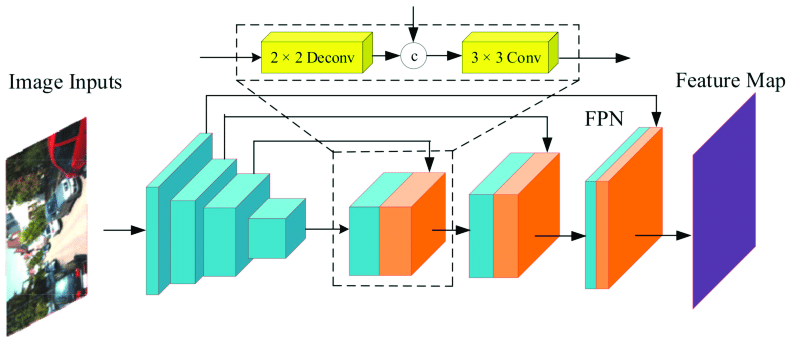
\includegraphics[scale=0.5]{Images/fpn_arch.png}
    \caption{Архітектура мереж FPN}
    \label{fpn_arch}
\end{figure}

FPN суттєво вплинули на різні реальні застосування, особливо в галузях, що
вимагають високоточного виявлення та сегментації об'єктів. В автономному
водінні FPN відіграють вирішальну роль в ідентифікації об'єктів, таких як
пішоходи, транспортні засоби та дорожні знаки, на основі зображень, отриманих з
камер, встановлених на транспортних засобах~\cite{liao2021}. Багатомасштабне
представлення об'єктів дозволяє з високою точністю виявляти як дрібні об'єкти,
такі як віддалені пішоходи, так і великі, наприклад, транспортні засоби, що
знаходяться поблизу. Ця можливість є життєво важливою для безпеки та надійності
автономних систем, де детальне розуміння навколишнього середовища має важливе
значення для навігації та прийняття рішень.

Загалом, універсальність та ефективність
Feature Pyramid Networks роблять їх потужним
інструментом у багатьох галузях, сприяючи
технологічному прогресу та підвищуючи точність
і надійність різних застосувань.

\section{Модель U-Net}

U-Net -- це архітектура згорткової нейронної мережі, розроблена в першу чергу
для біомедичної сегментації зображень. Представлена у
роботі~\cite{ronneberger2015}, U-Net набула значної популярності завдяки своїй
видатній продуктивності в різних задачах сегментації зображень. Архітектура
отримала назву <<U-Net>> через свою характерну U-подібну структуру, яка
складається зі шляху, що звужується (енкодер), і шляху, що розширюється
(декодер). Така конструкція дозволяє U-Net фіксувати як контекст, так і точну
локалізацію, що робить її особливо ефективною для сегментації невеликих і
складних структур на зображеннях (рис.~\ref{unet_arch}).

\begin{figure}[ht]
    \centering
    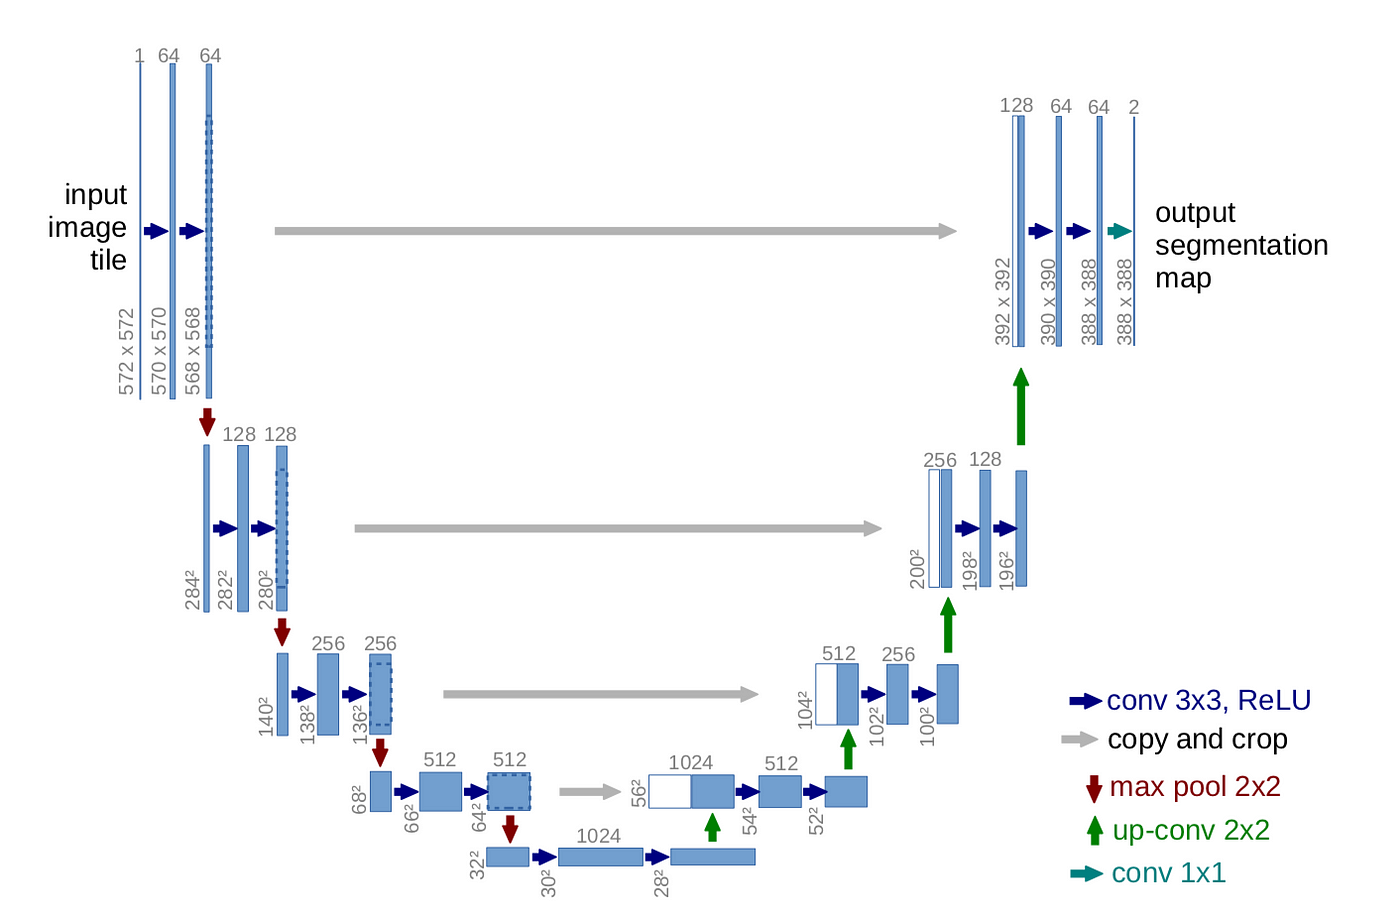
\includegraphics[scale=0.3]{Images/unet_arch.png}
    \caption{Архітектура U-Net}
    \label{unet_arch}
\end{figure}

Шлях згортання U-Net відповідає структурі типової згорткової
мережі, що складається з багаторазового застосування
згорткових шарів, за кожним з яких слідує активація
випрямленої лінійної одиниці (ReLU) та операція
максимального об'єднання для подальшої дискретизації.
Така послідовність операцій зменшує просторові розміри
карт ознак, одночасно збільшуючи їхню глибину,
що дозволяє мережі вивчати ієрархічні ознаки на різних
масштабах. Кожен крок на шляху звуження фіксує все
більш абстрактні представлення вхідного зображення,
які мають вирішальне значення для розуміння складних
закономірностей і контексту.

Розширювальний шлях є дзеркальним відображенням звужувального
шляху, але виконує протилежні операції. Він передбачає
збільшення вибірки карт об'єктів, зазвичай за допомогою
транспонованих згорток (також відомих як деконволюції),
для збільшення їхньої просторової роздільної здатності.
На кожному кроці збільшення вибірки мережа об'єднує
відповідні карти ознак зі шляху скорочення за допомогою
пропускних зв'язків. Ці з'єднання відіграють життєво
важливу роль в архітектурі U-Net, зберігаючи об'єкти з
високою роздільною здатністю, які в іншому випадку були
б втрачені під час процесу пониження дискретизації.
Поєднуючи ці детальні характеристики з високорівневою
семантичною інформацією, отриманою з глибших шарів,
мережа може точно окреслити межі об'єктів на зображенні.

Загалом, архітектура U-Net дозволяє ефективно
балансувати між необхідністю детальної локалізації
та контекстним розумінням, що робить його високоефективним
для задач сегментації зображень. Інноваційне використання
пропускних з'єднань і симетричний дизайн зробили її
популярним вибором у різних галузях, окрім біомедичної
візуалізації, включаючи аналіз супутникових зображень,
сільськогосподарський моніторинг тощо, де точна
сегментація має вирішальне значення.

U-Net знайшла широке застосування в різних галузях реального світу, а її
основні історії успіху пов'язані з біомедичною візуалізацією. У медичній
діагностиці U-Net використовується для сегментації анатомічних структур на
радіологічних зображеннях, таких як МРТ і КТ. Її здатність точно окреслювати
межі органів, тканин і патологічних ділянок, таких як пухлини, робить її
безцінною для допомоги радіологам у діагностиці та плануванні лікування.
Наприклад, в онкології U-Net допомагає ідентифікувати і вимірювати об'єм
пухлини, що має вирішальне значення для оцінки прогресування раку і планування
відповідних втручань.

Окрім медичної візуалізації, U-Net була успішно адаптована
для використання в екологічному і сільськогосподарському
моніторингу за допомогою аналізу супутникових і аерофотознімків
У цих сферах U-Net допомагає сегментувати різні типи
земного покриву, такі як ліси, міські території і водні
об'єкти, на основі супутникових знімків. Ця інформація
має вирішальне значення для моніторингу змін навколишнього
середовища, управління природними ресурсами і планування
міського розвитку. Крім того, в землеробстві U-Net
використовується для аналізу стану посівів шляхом сегментації
різних типів рослинності та виявлення ділянок, уражених
хворобами чи шкідниками~\cite{mou2018}. Ця програма дозволяє фермерам
здійснювати цілеспрямовані втручання, тим самим підвищуючи
врожайність і зменшуючи використання пестицидів.

\section{Модель DeepLabv3}

DeepLabv3~\cite{chen2017} -- це сучасна модель глибокого навчання для
семантичної сегментації зображень, яка полягає в поділі зображення на регіони
та визначенні категорії об'єктів, присутніх у кожному регіоні. Розроблена
Google Research, DeepLabv3 базується на попередніх версіях, DeepLabv1 і
DeepLabv2, і включає в себе кілька ключових інновацій, які підвищують її
продуктивність і точність. Одним з головних досягнень DeepLabv3 є використання
технології atrous convolution (також відомої як розширена згортка), яка
дозволяє ефективно збільшувати рецептивне поле без втрати роздільної здатності.
Ця методика дозволяє моделі захоплювати різномасштабну контекстну інформацію,
що має вирішальне значення для точної сегментації об'єктів різного розміру.

Ще однією важливою особливістю DeepLabv3 є використання
atrous spatial pyramid pooling (ASPP).
ASPP застосовує atrous convolution з різною швидкістю розширення
паралельно для захоплення інформації на різних масштабах. Цей
механізм вилучення різномасштабних ознак покращує здатність моделі
розпізнавати об'єкти на різних рівнях деталізації та просторових вимірів.
Крім того, DeepLabv3 інтегрує пакетну нормалізацію, яка стабілізує
і прискорює процес навчання шляхом нормалізації вхідних шарів.
Ця модель може бути реалізована з різними наперед тренованими енкодерами,
такими як ResNet, що ще більше підвищує її продуктивність
і адаптивність до різних завдань і наборів даних.

Крім того, модуль ASPP у DeepLabv3 ефективно фіксує різномасштабну
інформацію, досліджуючи особливості за допомогою фільтрів з
різними частотами дискретизації та полями зору. Експериментальні
результати моделі демонструють значні покращення порівняно з
попередніми версіями, досягнувши продуктивності 85,7\% на тестовому
наборі PASCAL VOC 2012 без необхідності постобробки DenseCRF.

DeepLabv3 є значним досягненням у галузі семантичної сегментації зображень,
пропонуючи надійну продуктивність і високу точність у різних додатках.
DeepLabv3 ефективно фіксує різномасштабну контекстну інформацію, що має
вирішальне значення для сегментації об'єктів різного розміру та складності.
Інтеграція пакетної нормалізації ще більше стабілізує процес навчання,
підвищуючи ефективність та надійність моделі.

\section{Функція втрат Dice Loss}

Dice Loss -- це популярна функція втрат, яка використовується переважно в
галузі сегментації зображень, особливо в аналізі медичних
зображень~\cite{zhang2021}. Вона походить від коефіцієнта Сьоренсена-Дайса,
статистичної міри, яка кількісно оцінює схожість між двома наборами. Dice Loss
особливо ефективна для задач, де набір даних незбалансований, наприклад, для
сегментації невеликих структур, таких як пухлини на медичних зображеннях.
Основною перевагою Dice Loss є його здатність впоратися з таким дисбалансом,
безпосередньо максимізуючи перекриття між прогнозованою сегментацією і базовою
істиною, що має вирішальне значення для отримання точних результатів
сегментації.

Математично коефіцієнт Дайса визначається як подвоєна
площа перекриття між прогнозованою сегментацією
і базовим зображенням, поділена на загальну кількість
пікселів на обох зображеннях. В контексті сегментації
зображень, втрати Дайс формулюються як одиниця мінус
коефіцієнт Дайс, який перетворює міру схожості у
функцію втрат, яку можна мінімізувати. Формулу для
Dice Loss можна записати як:

\begin{equation*}
    DL = 1 - \frac{2|A \cap B|}{|A| + |B|},
\end{equation*}
де A -- набір пікселів у прогнозованій сегментації,
а B -- набір пікселів у істинній сегментації.
Мінімізуючи Dice Loss, модель заохочується
до максимізації перекриття між прогнозованою
та фактичною сегментацією, таким чином покращуючи
точність сегментації.

Включення Dice Loss у процес навчання дозволяє моделі
навчитися вловлювати складні просторові взаємозв'язки
та дрібні деталі, присутні на супутникових знімках,
що призводить до більш точних результатів сегментації.

Крім того, використання Dice Loss допомагає
пом'якшити дисбаланс класів, який часто зустрічається
в задачах сегментації супутникових знімків. Супутникові
знімки зазвичай містять великі ділянки однорідного фону,
що перемежовуються з меншими регіонами, які становлять
інтерес. Dice Loss вирішує цю проблему,
призначаючи вищі штрафи за неправильну
класифікацію класів меншин, тим самим сприяючи
збалансованій сегментації різних типів земного покриву.
Загалом, інтеграція Dice Loss для
сегментації супутникових знімків підвищує
здатність моделей машинного навчання видобувати значущу
інформацію з супутникових знімків, полегшуючи різні
подальші застосування в таких галузях, як моніторинг
довкілля, сільське господарство і міське планування.

\section{Функція втрат Focal Loss}

Focal Loss -- це функція втрат, запропонована в роботі~\cite{lin2017} для
усунення екстремального дисбалансу класів, що виникає під час навчання
детекторів щільних об'єктів. Цей дисбаланс виникає, коли в наборі даних значно
більше простих негативних прикладів, ніж позитивних. Focal Loss має на меті
зменшити втрати, пов'язані з добре класифікованими прикладами, і зосередити
навчання на важких, неправильно класифікованих прикладах. Це досягається
додаванням модулюючого множника $(1 - p_t)^\gamma$ до стандартної перехресної
ентропійної втрати (cross-entropy loss), де $p_t$ представляє прогнозовану
ймовірність класу базової істини, а $\gamma \geq 0$ -- фокусний параметр.

Таким чином, формула для Focal Loss має наступний вигляд:

\begin{equation*}
    FL(p_t) = -(1-p_t)^\gamma log(p_t).
\end{equation*}

Основна ідея Focal Loss полягає в тому,
щоб зменшити внесок простих прикладів під час навчання,
таким чином запобігаючи їхньому перевантаженню датчика.
Регулюючи параметр фокусування $\gamma$, можна контролювати швидкість,
з якою легкі приклади втрачають вагу. Коли приклад
невірно класифіковано і $p_t$ малий, модулюючий коефіцієнт близький до
1, і втрати не впливають. Однак, коли $p_t$ наближається до 1,
коефіцієнт зменшується до 0, що призводить до зменшення втрат
для добре класифікованих прикладів.

Focal Loss призначена для обробки дисбалансу класів безпосередньо через функцію
втрат, на відміну від традиційних методів, таких як двоступеневі детектори, які
покладаються на каскадні механізми і зміщену вибірку. Зосереджуючись на важких
негативних прикладах, Focal Loss дозволяє ефективно навчати на всіх прикладах
без необхідності вибірки або схем перезважування.

Експериментальні результати, представлені в роботі~\cite{lin2017},
демонструють ефективність Focal Loss у навчанні високоточного
одноетапного детектора об'єктів під назвою RetinaNet.
Focal Loss перевершує попередні методи боротьби з дисбалансом класів,
такі як евристика вибірки або навчання на складних прикладах,
і дозволяє детектору досягти кращої точності, зберігаючи при цьому швидкість.

\subsection*{Висновки до розділу 2}
Отже, у даному розділі було проведено огляд моделей машинного навчання
та функцій втрат. Було досліджено три сучасні архітектури мереж: FPN, U-Net, та DeepLabv3 які вже
тривалий час показують свою ефективність у задачах сегментації зображень,
в основному, на медичних знімках. Досліджуваними функціями втрат були
Dice Loss і Focal Loss, які теж часто використовується у задачах сегментації. У ході
дослідження було виявлено, що дані інструменти гарно підійдуть для
сегментації кратерів на супутникових знімках.
%!TEX root = ../thesis.tex
\chapter{Розробка та порівняльний аналіз моделей машинного навчання навчання}
\label{chap:practice}

\section{Підготовка датасету}

Для формування датасету використано два основних джерела даних:
супутникове зображення та відповідну маску з розміченими кратерами.
Важливо зазначити, що в межах даної роботи використані дані,
сформовані науковим колективом кафедри ММАД.
Початковий датасет був фрагементований
на патчі розміром 128x128 пікселів. Такий розмір був обраний довільно,
моделі, представлені у даній роботи, підтримують зображення будь якого
розміру, з умовою, що розширення ділиться на 32 націло.
Відбір
патчів для подальшої обробки відбувався на підставі критерію, згідно
з яким у вибраних патчах область, що відповідала масці, становила не
менше 10\% загальної площі. Цей підхід сприяє виокремленню
суттєвих особливостей і забезпечує відсутність у датасеті
зображень, які не мають достатнього для навчання матеріалу. У результаті цього етапу формування
було отримано 1000 патчів. Наступним кроком було розділення
отриманого датасету на тренувальні, валідаційні та тестові підмножини
відповідно у відношенні 80\%:10\%:10\%. Ця стратегія розподілу дозволяє
забезпечити ефективне навчання моделі та об'єктивну оцінку її продуктивності
на випробувальних даних. Програмна реалізація даного модулю представлена у додатку А.1.

\section{Реалізація моделей}

У рамках дослідження використано три широко відомі моделі для
сегментації зображень: FPN, U-Net та DeepLabv3,
усі з базовою згортковою архітектурою ResNet-34.
ResNet-34 -- це глибока згорткова нейронна мережа, навчена на наборі
даних CIFAR-10~\cite{he2015}. Це частина сімейства ResNet,
яке вирішило проблему зникнення градієнтів у глибоких
нейронних мережах, що дозволяє ефективно навчати набагато
глибші мережі. Основна інновація ResNet-34 полягає
у використанні залишкового навчання. Замість того, щоб
вивчати пряме відображення від входу до виходу, залишкові
мережі вивчають різницю (або залишок) між входом і виходом.
Цей підхід реалізується за допомогою коротких з'єднань,
які оминають один або декілька шарів, що дозволяє мережі
вивчати залишкові функції з посиланням на входи шарів.

Архітектура ResNet-34 складається з 34 згорткових шарів,
організованих у серії залишкових блоків. Кожен блок містить
два згорткових шари, за якими слідує коротке з'єднання,
що додає вхід блоку до його виходу. Мережа починається
з початкового згорткового шару, за яким слідує шар
максимального об'єднання, а потім проходить через
чотири етапи залишкових блоків. Ці етапи містять 3, 4, 6
і 3 блоки відповідно, причому на кожному етапі кількість
фільтрів збільшується і подвоюється на кожному переході.
Мережа завершується глобальним середнім об'єднуючим шаром
і повністю з'єднаним шаром для цілей класифікації.

ResNet-34 показала чудову продуктивність у різних задачах розпізнавання
зображень, значно зменшивши помилки навчання завдяки вирішенню проблеми
зникаючого градієнта, яка є поширеною в глибоких мережах.

Для реалізації обраних моделей для завдання сегментації
зображень, а також використання функцій втрат Dice Loss і Focal Loss,
було використано пакет Segmentation Models
PyTorch~\cite{iakubovskii2019}, який
надає готові реалізації різноманітних архітектур
нейронних мереж для сегментації зображень на базі
бібліотеки PyTorch. Цей пакет дозволяє швидко та зручно
використовувати високоякісні моделі, а також зручно
налаштовувати параметри навчання та валідації.
Використання готових реалізацій у пакеті спрощує
процес розробки та дозволяє зосередитися на розв'язанні
основної задачі без необхідності вирішувати деталі
реалізації моделей.

Додатково, для забезпечення ефективного та
структурованого процесу навчання моделей та відладки
коду, використовувалася бібліотека PyTorch Lightning~\cite{falcon2019}.
PyTorch Lightning надає високорівневий інтерфейс для
навчання нейронних мереж на базі PyTorch, що дозволяє
зосередитися на архітектурі та параметрах моделі,
відділивши їх від деталей навчання. Завдяки цьому,
можна зручно використовувати різноманітні техніки
навчання, такі як автоматичне зберігання моделі,
відстеження метрик, розподіл тренування на різні
пристрої та багато іншого. Використання PyTorch
Lightning сприяло підвищенню продуктивності розробки
та навчання моделей для задачі сегментації зображень.
Програмна реалізація основного модулю програми наведену у додатку А.2.

Для об'єктивного порівняння точності моделей,
використаних у дослідженні, було застосовано метрику
Intersection over Union (IoU) на валідаційному датасеті.
Ця метрика вимірює ступінь перекриття між прогнозованою
та реальною сегментаційними масками і дозволяє отримати
об'єктивну оцінку якості сегментації. Формула IoU наступна:
\begin{equation*}
      \text{IoU} = \frac{|A \cap B|}{|A \cup B|}.
\end{equation*}

Також моделі були оцінени на тестовому датасеті, звідки отримано
значення метрик recall (повнота), precision (точність) і F1.

Повнота, також відома як чутливість або частота
істинних позитивних результатів, вимірює частку фактичних
позитивних результатів, які правильно ідентифіковані моделлю.
Формула повноти виглядає так:
\begin{equation*}
      \text{Recall} = \frac{TP}{TP + FN},
\end{equation*}
де $TP$ (True Positives) -- кількість
правильно передбачених позитивних пікселів,
а $FN$ (False Negatives) -- кількість фактичних
позитивних результатів, які були помилково
класифіковані як негативні.

Точність, також відома як позитивна прогностична цінність,
вимірює частку позитивних ідентифікацій, які
насправді є правильними.
Формула для точності має вигляд:

\begin{equation*}
      \text{Precision} = \frac{TP}{TP + FP},
\end{equation*}
де $FP$ (False Positives) -- кількість негативних пікселів,
які були помилково класифіковані як позитивні.

Оцінка F1 -- це середнє гармонійне значення точності та
повноти, що забезпечує єдину метрику,
яка збалансовує обидва показники. Вона
особливо корисний, коли класи незбалансовані,
оскільки враховує як хибнопозитивні, так і
хибнонегативні спрацьовування. Формула для
оцінки F1 має вигляд:

\begin{equation*}
      \text{F1} = 2 \times \frac{\text{Precision} \times \text{Recall}}{\text{Precision} + \text{Recall}}.
\end{equation*}
Ця метрика приймає значення від 0 до 1, де
вищий показник вказує на кращий баланс між
точністю та повнотою.

\section{Порівняльний аналіз моделей машинного навчання}

Спираючись на графік, зображений на рис.~\ref{iou_comp},
можна сказати, що моделі, які навчалися з Dice Loss,
навчаються більш стабільно, ніж ті, у яких функцією
втрат виступає Focal Loss.
Причинами цього можуть бути фактори, наведені нижче.

\begin{itemize}

      \item Чутливість моделі до складних прикладів:
            Focal Loss надає більшої ваги складним прикладам,
            які модель намагається правильно класифікувати.
            Таке підвищене фокусування може призвести до більш
            значних коливань у прогнозах моделі, особливо на
            ранніх стадіях навчання, коли параметри моделі все
            ще оптимізуються. Як наслідок, метрика IoU, яка є
            чутливою до якості прогнозів, може демонструвати
            більшу варіабельність і виглядати хвилясто.
      \item Швидкість навчання та динаміка оптимізації:
            вибір швидкості навчання та інших гіперпараметрів
            оптимізації може впливати на стабільність процесу
            навчання. Висока швидкість навчання може спричинити
            сильніші коливання параметрів моделі, що призведе до
            нестабільних показників ефективності. Навіть при добре
            підібраній швидкості навчання, притаманна динаміка
            фокусування на складних прикладах
            може внести нестабільність у процес навчання, що
            призведе до хвилястої кривої IoU.
      \item Ефекти регуляризації: методи регуляризації,
            такі як пулінг або доповнення даних, які
            часто використовуються для запобігання надмірному
            пристосуванню, можуть внести додаткову варіативність
            у навчальний процес. У поєднанні з Focal Loss,
            яка вже змінює оновлення градієнта, щоб зосередитися
            на важких прикладах, ця мінливість може відображатися
            на метриці IoU, роблячи її менш стабільною.

\end{itemize}

\begin{figure}[ht]
      \centering
      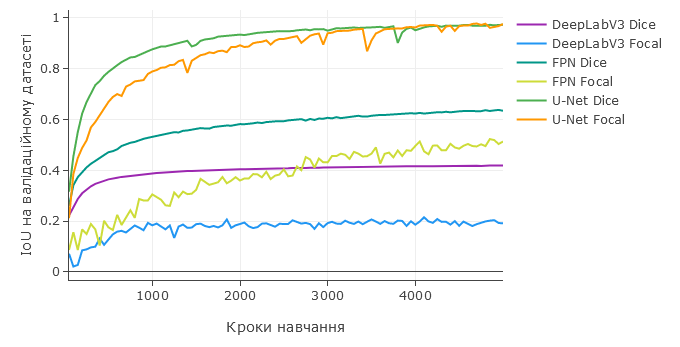
\includegraphics[scale=0.8]{Images/iou_comp.png}
      \caption{Порівняння значення IoU під час навчання}
      \label{iou_comp}
\end{figure}

За даними табл.~\ref{int_comp}, можна зробити наступні висновки.
Найбільш ефективною моделлю виявилась U-Net, при чому і з використанням
Dice Loss, і з використанням Focal Loss. Це свідчить про те, що
архітектура даної моделі найкраще підходить для вирішення поставленої
задачі, а модель добре підлаштувалась під навчальні дані. Високі показники
моделі на тестовому датасеті показають, що модель не перетренована.

Найгірше себе проявила модель DeepLabv3. Вона не тільки має найменші показники
повноти, точності та F1, але й має найбільший час навчання, майже вдвічі довше,
ніж інші представлені моделі.

Ще одним висновком є те, що моделі, які навчались з використанням Dice Loss,
показують кращі результати за ті, що навчались з використанням Focal Loss.

\begin{table}[ht]
      \setfontsize{12pt}
      \caption{Порівнняня метрик моделей глибокого навчання}
      \label{int_comp}
      \centering
      \begin{tabular}{|c|c|c|c|c|c|c|}
            \hline
            Функція втрат               & Назва моделі & Recall & Precision & F1   & IoU  & Час навчання (хв.) \\ \hline
            \multirow{3}{*}{Dice Loss}  & FPN          & 0.85   & 0.71      & 0.77 & 0.63 & 29.31              \\ \cline{2-7}
                                        & U-Net        & 0.98   & 0.99      & 0.99 & 0.97 & 34.37              \\ \cline{2-7}
                                        & DeepLabv3    & 0.78   & 0.47      & 0.59 & 0.42 & 53.86              \\ \hline
            \multirow{3}{*}{Focal Loss} & FPN          & 0.64   & 0.73      & 0.68 & 0.51 & 37.15              \\ \cline{2-7}
                                        & U-Net        & 0.98   & 0.99      & 0.99 & 0.97 & 40.1               \\ \cline{2-7}
                                        & DeepLabv3    & 0.22   & 0.58      & 0.32 & 0.19 & 54.48              \\ \hline
      \end{tabular}
\end{table}

На рис.~\ref{image_and_gt} зображений приклад знімку і істинної маски,
взятий з тестового датасету. На цьому прикладі були продемонстровані
прогнозовані маски моделей, навчених з використанням Dice Loss (рис.~\ref{pred_dice_comp})
і Focal Loss (рис.~\ref{pred_focal_comp}).

\begin{figure}[ht]
      \centering
      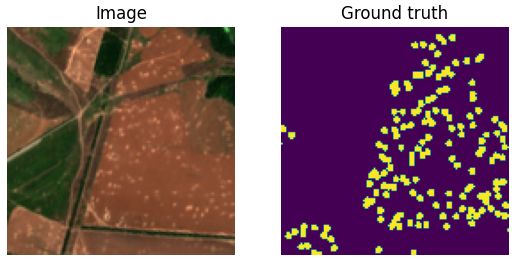
\includegraphics[scale=1]{Images/image_and_gt.png}
      \caption{Приклад знімку і істинної маски з тестового датасету}
      \label{image_and_gt}
\end{figure}

\begin{figure}[ht]
      \centering
      \begin{subfigure}[b]{0.33\textwidth}
            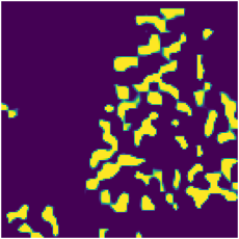
\includegraphics[scale=0.75]{Images/fpn_dice_pred.png}
            \caption{FPN}
      \end{subfigure}%
      \begin{subfigure}[b]{0.33\textwidth}
            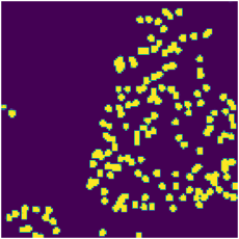
\includegraphics[scale=0.75]{Images/unet_dice_pred.png}
            \caption{U-Net}
      \end{subfigure}
      \begin{subfigure}[b]{0.33\textwidth}
            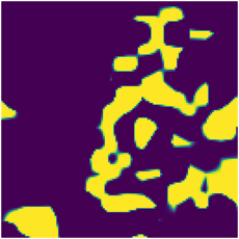
\includegraphics[scale=0.75]{Images/deeplab_dice_pred.png}
            \caption{DeepLabv3}
      \end{subfigure}

      \caption{Порівняння прогнозованих масок моделей з функцією втрат Dice Loss}
      \label{pred_dice_comp}
\end{figure}

\begin{figure}[ht]
      \centering
      \begin{subfigure}[b]{0.33\textwidth}
            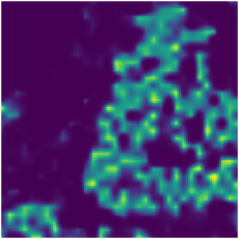
\includegraphics[scale=0.75]{Images/fpn_focal_pred.png}
            \caption{FPN}
      \end{subfigure}%
      \begin{subfigure}[b]{0.33\textwidth}
            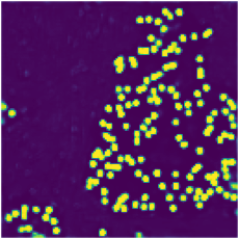
\includegraphics[scale=0.75]{Images/unet_focal_pred.png}
            \caption{U-Net}
      \end{subfigure}
      \begin{subfigure}[b]{0.33\textwidth}
            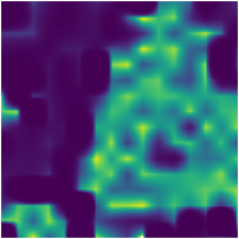
\includegraphics[scale=0.75]{Images/deeplab_focal_pred.png}
            \caption{DeepLabv3}
      \end{subfigure}

      \caption{Порівняння прогнозованих масок моделей з функцією втрат Focal Loss}
      \label{pred_focal_comp}
\end{figure}

Зважаючи на представлені приклади, наочно видно переваги Dice Loss
над Focal Loss. Хоча U-Net має приблизно ідентичні показники
ключових метрик, прогнозована маска у моделі, як навчалась з Dice Loss,
має чіткіші межі кратерів і не має відхілень, на відміну від моделі
з Focal Loss. Результати інших двох моделей, FPN та DeepLabv3,
суттєво відрізняються в залежності від функції втрат. Результати
з Dice Loss набагато чіткіші, хоча й мають проблеми з
розрізненнями індивідуальних кратерів. Причинами такої поведінки
є наступнє:

\begin{itemize}

      \item Dice Loss дуже чутлива до просторового перекриття між прогнозованими та
            фактичними сегментами. Ця чутливість спонукає модель створювати більш точні
            прогнози як за формою, так і за розташуванням, що має вирішальне значення для
            задач, де потрібна точна сегментація.
      \item У випадках, коли об'єкти сегментації є
            невеликими та розрідженими, Dice Loss може
            бути особливо ефективною. Вона гарантує,
            що модель приділяє належну увагу малим регіонам,
            уникаючи зміщення в бік більших регіонів, яке може
            виникнути з іншими функціями втрат, такими як Cross-Entropy Loss і Focal Loss.
      \item Dice Loss за своєю суттю врівноважує внесок суттєвих класів і фону. У задачах
            сегментації, особливо при роботі з медичними зображеннями або виявленні рідких
            об'єктів, об'єкт інтересу часто займає набагато меншу площу порівняно з фоном.
            Dice Loss відповідним чином масштабує важливість суттєвих класів, гарантуючи,
            що невеликим структурам надається більше значення в процесі навчання.

\end{itemize}

Хоча Focal Loss ефективна для обробки дисбалансу
класів і фокусування на складних прикладах, вона
не оптимізує безпосередньо перекриття між прогнозованими
і фактичними сегментами. Іноді це може призвести до менш
оптимальної продуктивності в задачах сегментації порівняно
з Dice Loss, яка спеціально розроблена для максимізації перекриття
по регіонах.

У контексті даної роботи, U-Net краще справляється з
сегментацією кратерів. U-Net була спеціально розроблена
для сегментації біомедичних зображень, де часто зустрічаються
невеликі об'єкти. Її архітектура, що характеризується симетричними
кодерно-декодерними шляхами з пропускними з'єднаннями,
чудово зберігає просторову інформацію та захоплює дрібні деталі.
Пропускні з'єднання допомагають зберегти характеристики
високої роздільної здатності від кодера і поєднати їх з
характеристиками декодера, що має вирішальне значення для
точної сегментації дрібних об'єктів.

В той же час, і DeepLabV3, і FPN передбачають багаторазове
зменшення вибірки для вилучення об'єктів, що може призвести
до втрати просторової роздільної здатності. Хоча ці
архітектури використовують методи відновлення просторової
інформації (наприклад, збільшення вибірки і використання
карт об'єктів з вищою роздільною здатністю), початкова
втрата деталей може вплинути на якість сегментації для
невеликих об'єктів. Архітектура U-Net, з її орієнтацією на
збереження інформації з високою роздільною здатністю завдяки
використанню пропускних з'єднань, краще підходить для
вирішення цієї проблеми.

\section*{Висновки до розділу 3}

Отже, у даному розділі було
описано процес розробки та проведено порівняльний аналіз
моделей машинного навчання для розв'язання задачі
сегментації кратерів на супутникових зображеннях.
Датасет, який початково
складався із одного знімку та відповідної розміченої маски, було
поділено на випадкові патчі розміру 128x128, і обрані ті з них,
де маска складала хоча б 10\% від загальної картинки.
Таким чином, було отримано достатньо даних для навчання, валідації та
тестування обраних моделей. Імплементація моделей та функції втрат відбувалась за допомогою
бібліотек Segmentation Models PyTorch і PyTorch Lightning, які
значно спростили побудову та навчання моделей.

Найбільш ефективною моделлю виявилась U-Net з використанням Dice Loss,
а найменш ефективною -- DeepLabv3 з використанням Focal Loss.
U-Net дає змогу точно визначити місцеположення кратерів, в той час
як інші дві моделі можуть надавати лише приблизні зони впливу,
а окремі кратери виділяються дуже рідко.
Також, варто зазначити, що моделі, які навчалися з Dice Loss
показують кращі і більш стабільні результати ніж ті,
що навчались з Focal Loss.

% Створюємо висновки
\conclusions
%!TEX root = ../thesis.tex
% створюємо Висновки до всієї роботи
Отже, у даній роботі було проведено аналіз та порівняння методів
машинного навчання для розв'язання задачі сегментації кратерів
на супутникових знімках.

У ході виконання даної роботи був проведений аналіз опублікованих
джерел за тематикою виявлення кратерів на супутникових
знімках, який показав, що тема є актуальною на сьогоднішній день.
У приведених роботах використовувалися різні підходи, а саме MPP, CNN, та
методи, засновані на використанні статистичних показників.
MPP показав свою ефективність у розв'язуванні цієї задачі, особливо
за умов, коли немає розміченої маски, або коли даних недостатньо для
тренування більш складної CNN моделі. Методи, засновані
на статистичних показниках теж потребують менше даних за CNN,
але потрібні знімки, розподілені у часі, що може ускладнити успішне використання
цього методу.
У той же час, якщо даних достатньо,
то CNN дає більш точні результати.

У ході формалізації завдання було дано визначення поняттю кратера,
описані вхідні дані, кроки методології та метрики, за якими будуть
порівнюватися моделі машинного навчання.

Наступним кроком дослідження був огляд моделей і функцій втрат.
Було досліджено три сучасні архітектури мереж: FPN, U-Net, та DeepLabv3 які вже
тривалий час показують свою ефективність у задачах сегментації зображень,
в основному, на медичних знімках. Досліджуваними функціями втрат були
Dice Loss і Focal Loss, які теж часто використовується у задачах сегментації. У ході
дослідження було виявлено, що дані інструменти гарно підійдуть для
сегментації кратерів на супутникових знімках.

Далі було підготовано датасет та імплементовано моделі. Датасет, який початково
складався із одного знімку та відповідної розміченої маски, було
поділено на випадкові патчі розміру 128x128, і обрані ті з них,
де маска складала хоча б 10\% від загальної картинки.
Таким чином, було отримано достатньо даних для навчання, валідації та
тестування обраних моделей. Імплементація моделей та функції втрат відбувалась за допомогою
бібліотек Segmentation Models PyTorch і PyTorch Lightning, які
значно спростили побудову та навчання моделей.

Наприкінці, було проведено порівняльний аналіз моделей машинного навчання.
Найбільш ефективною виявилась U-Net з використанням Dice Loss,
а найменш ефективною -- DeepLabv3 з використанням Focal Loss.
U-Net дає змогу точно визначити місцеположення кратерів, в той час
як інші дві моделі можуть надавати лише приблизні зони впливу,
а окремі кратери виділяються дуже рідко.
Також, варто зазначити, що моделі, які навчалися з Dice Loss
показують кращі і більш стабільні результати ніж ті,
що навчались з Focal Loss.

Практичні результати роботи були висвітлені на XXII Всеукраїнській
науково-практичній конференції студентів, аспірантів
та молодих вчених на базі Навчально-наукового Фізико-технічного
інституту Національного технічного університету України
<<Київський політехнічний інститут імені Ігоря Сікорського>>.

% Додаємо бібліографію
%%%%%%% Якщо ви не використовуєте bibtex, оце все треба закоментувати звідси...
\defbibenvironment{bibliography}
{\list
  {\printfield[labelnumberwidth]{labelnumber}}
  {\setfontsize{14}%
  }}
{\endlist}
{\item}

\printbibliography[heading=bibintoc,title={Список використаних джерел}]
%%%%%%% ...по осюди

% Якщо у вас виникли проблеми з бібтехом (у мене, наприклад, виникли), то замість бібтеху
% можна використати менш приємний, але завжди працюючий спосіб: вписати та оформити бібліографію вручну
% Для цього закоментуйте команду \printbibliography та розкоментуйте наступний рядок
% VVV оцей рядок розкоментуйте VVV
%%!TEX root = ../thesis.tex
% створюємо список використаної літератури
\begin{thebibliography}
    \bibitem{sad}
    asda

    \bibitem{dca}
    asd [Електронний ресурс]. --- Режим доступу: \url{dsf}.

\end{thebibliography}

% ^^^ оцей-оцей ^^^
% Бібліографія вноситься у файл "w2_bibliography.tex"

%%% А це взагалі перестало працювати :(
%\bibliographystyle{ugost2008}
%\bibliography{thesis}

% Створюємо додатки (дивись у файли додатків для необхідних пояснень)
% Якщо ви маєте меншу або більшу кількість додатків, модифікуйте наступні 
% рядки відповідним чином
% Якщо ви не маєте додатків, просто закоментуйте наступні рядки
%!TEX root = ../thesis.tex
\append{Лістинги програм}
\label{appendix:A}

\section{Програма для фрагментації знімку і маски}
\lstinputlisting[language=python, basicstyle=\small]{Code/dataset_preparer.py}

\section{Основна програма}
\lstinputlisting[language=python, basicstyle=\small]{Code/main.py}

% Нарешті
\end{document}